\documentclass[a4paper]{ltjsarticle}
\usepackage{base, math_phys}

\makeatletter
\long\def\@makefntext#1{\parindent 1em\noindent
\@hangfrom{\hbox to 1.8em{\hss$^{\@thefnmark}$}}#1}
\makeatother
\theoremstyle{definition}
\newtheorem{dfn}{定義}[section]
\newtheorem{thm}[dfn]{定理}
\newtheorem{prop}[dfn]{命題}
\newtheorem{cor}[dfn]{系}
\newtheorem{lem}[dfn]{補題}
\newtheorem{ex}[dfn]{例}
\newtheorem{rem}[dfn]{注意}
\newtheorem{que}{問}[section]
\newtheorem{ans}{解答}[section]

\usepackage{float}
\newcommand{\disp}[1]{\displaystyle{#1}}
\usepackage{fancybox}
\usepackage{footnote}
\usepackage{multicol}
\usepackage{tcolorbox}
\tcbuselibrary{raster,skins}
\newtcolorbox{mybox}{%
colback=blue!10!white,
colframe=white,
arc=5pt,
outer arc=3pt}
\tcbuselibrary{raster,skins}
\newtcolorbox{mysubbox}{%
colback=white,
colframe=black,
arc=1pt,
outer arc=2pt}
\renewcommand{\arraystretch}{2.3}
\newcommand{\1}{$\star$}
\newcommand{\2}{$\star\star$}
\newcommand{\3}{$\star\star\star$}
\newcommand{\4}{$\star\star\star\star$}
\newcommand{\card}[1]{\mathrm{Card}~#1}
\newcommand{\GCD}{\mathrm{GCD}~}
\newcommand{\defarrow}{\overset{\text{def}}{\Longleftrightarrow}}
\newcommand{\add}[1]{\textcolor{red}{#1}}
\newcommand{\erase}[1]{\sout{#1}}
\newcommand{\mylim}[3]{\lim_{#1→#2}#3}
\newcommand{\myint}[2]{\int_{#1}^{#2}}
\newcommand{\sinx}{\sin x}
\newcommand{\cosx}{\cos x}
\newcommand{\tanx}{\tan x}
\newcommand{\logx}{\log x}
\newcommand{\II}{I\hspace{-1.2pt}I}
\newcommand{\coshx}{\cosh x}
\newcommand{\sinhx}{\sinh x}
\newcommand{\tanhx}{\tanh x}
\renewcommand{\ker}{\mathrm{Ker}~}
\newcommand{\euvect}[2]{\bm{#1}=(#1_1,#1_2,\ldots ,#1_{#2})}
\newcommand{\myrank}[1]{\mathrm{Rank}\; #1}
\newcommand{\mydim}[1]{\mathrm{dim}\; #1}
\newcommand{\dydx}{\frac{dy}{dx}}
\newcommand{\cover}[1]{\maketitle
\setcounter{tocdepth}{#1}
\tableofcontents
\thispagestyle{empty}
\addtocounter{page}{-1}
\newpage}
\newcommand{\hint}[1]{\footnote{ヒント:#1}}
\newcommand{\q}[1]{(#1)~}
\newcommand{\inp}[2]{(\bm{#1}~,~\bm{#2})}
\newcommand{\emp}{\hspace{50mm}}

\title{3章~第2節 極座標と極方程式}
\author{2年\underline{  }組 出席番号:\underline{   } 氏名:\underline{            }}
\date{}
\begin{document}

\maketitle
\thispagestyle{empty}
\section{極座標}
本時は,平面上の点を表す新たな方法として極座標と呼ばれるものを導入する.実は,極座標の考え方は極形式と本質的に同じである.まずは,極形式の復習をしよう.
\subsection{復習:極形式}
\begin{multicols}{2}
    複素数$z=a+bi$を考える.ただし,$a,b$は実数である.$z$に対応する複素数平面上の点を$P$とし,右の図のように,$OP=r$,実軸の正の方向となす角度を$\theta$とするとき,
    \[z=r(\cos\theta+i\sin\theta)\]
    表される.これを$z$の\underline{\textbf{極形式}}といった.\\
    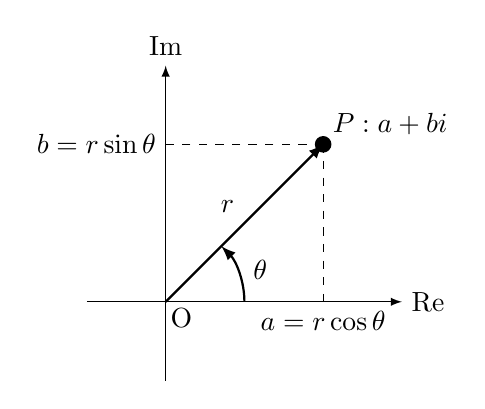
\begin{tikzpicture}[scale=2, >=latex]

        % Draw axes
        \draw[->] (-0.5,0) -- (1.5,0) node[right] {$\mathrm{Re}$}; % Real axis
        \draw[->] (0,-0.5) -- (0,1.5) node[above] {$\mathrm{Im}$}; % Imaginary axis
      
    
      
        % Draw the complex number as a point
        \fill (1,1) circle (1.5pt) node[above right] {$P:a+bi$};
      
        % Draw the vector from origin to the point
        \draw[->, thick] (0,0) -- (1,1) node[midway, above left] {$r$};
      
        % Draw the radius label
        \draw[->, thick] (1/2,0) arc[start angle=0, end angle=45, radius=0.5cm];
        \node at (0.6, 0.2) {$\theta$};
      
        % Labels for the coordinates
        \draw[dashed] (1,1) -- (1,0) node[below] {$a=r\cos\theta$};
        \draw[dashed] (1,1) -- (0,1) node[left] {$b=r\sin\theta $};
      \node at (0.1,-0.1){O};
      
      \end{tikzpicture}
\end{multicols}
\subsection{極座標}
複素数$z$の極形式からわかるように,複素数平面上の点は
\begin{itemize}
    \item  \\
    \item  
\end{itemize}
によって記述できる.これを,いつもの$xy$-平面に適用したものが極座標である.\\[5pt]
\newpage
\thispagestyle{empty}

\begin{tcolorbox}[top=2mm, left=5mm, bottom=2mm,
    sharp corners]

        \begin{multicols}{2}
            \textbf{定義.}\\[3pt]
        平面上に点Oと半直線$OX$を入れる.この平面上の点Pに対し,$\ns{OP}=r$,OXからOPへ測った角を$\theta$とする(右図参照).\\
        すると,Pの位置は$r,\theta$の大きさで定まる.点Pの位置を$(r,\theta)$と表したものを$P$の\underline{\textbf{極座標}}という.\\[3pt]
        また,このときの点Oを\underbar{\textbf{極}},$OP$を\underbar{\textbf{動径}},半直線$OX$を\underline{\textbf{始線}},$\theta$を\underline{\textbf{偏角}}という.\\[30pt]
        \begin{figure}[H]
            \centering
        \begin{tikzpicture}[scale=1.3, >=latex]
            % Axis labels
            \draw[->] (0,0) -- (3,0) node[below] {$X$}; % x-axis

            \draw[->] (0,0) -- (2,2.5) node[right]{$P:(r,\theta)$};

            \node at (1,1.6){$r$};
           
            % Draw the radius label
            \draw[->, thick] (1,0) arc[start angle=0, end angle=50, radius=1cm];
            \node at (1.2, 0.6) {$\theta$};

            % Polar center label
            \node[below left] at (0,0) {O};

            %name
            \node at (1.5,-0.3){始線};
           \node at (0.5,1.8){動径};
           \node at (-0.2,-0.5){極};
           \node at (1.6,0.9){偏角};
          
          \end{tikzpicture}
        \end{figure}
        \end{multicols}
  \end{tcolorbox}
 
    \noindent \textbf{問題1.}\\
    \noindent 極座標が
    \[\ns{A}=\left(1,\frac\pi2\right),\ns{B}=\left(2,\frac67\pi\right),\ns{C}=\left(3,-\frac{\pi}{3}\right)\]である点を図示せよ.\\[5pt]\textbf{解答欄.}
    \begin{figure}[H]
        \centering
    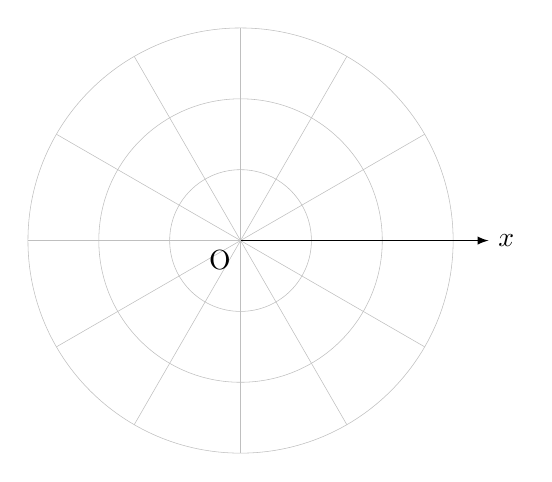
\begin{tikzpicture}[scale=0.9, >=latex]

        % Draw the polar grid (3 concentric circles and radial lines)
        \draw[very thin, gray!50] (0,0) circle (1);
        \draw[very thin, gray!50] (0,0) circle (2);
        \draw[very thin, gray!50] (0,0) circle (3);
      
        % Radial lines
        \foreach \angle in {0,30,...,330} {
          \draw[very thin, gray!50] (0,0) -- (\angle:3);
        }
      
        % Axis labels
        \draw[->] (0,0) -- (3.5,0) node[right] {$x$}; % x-axis
        \draw[very thin, gray!50] (0,-3) -- (0,3) ; % y-axis
      
        % Polar center label
        \node[below left] at (0,0) {O};
      
      \end{tikzpicture}
    \end{figure}
\begin{multicols}{2}

    \noindent \textbf{直交座標との関係.}\\[3pt]
    \noindent 極座標が
    極座標と直交座標を重ね合わせると,直交座標$(x,y)$と極座標$(r,\theta)$の間には次の関係があることがわかる.
    \begin{equation*}
        \begin{cases*}
            x= r \cos \theta & \\
            y= r \sin \theta &
        \end{cases*}
    \end{equation*}
            \\
    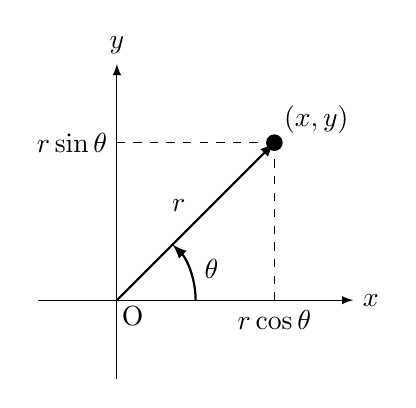
\begin{tikzpicture}[scale=2, >=latex]

        % Draw axes
        \draw[->] (-0.5,0) -- (1.5,0) node[right] {$x$}; % Real axis
        \draw[->] (0,-0.5) -- (0,1.5) node[above] {$y$}; % Imaginary axis
      
    
      
        % Draw the complex number as a point
        \fill (1,1) circle (1.5pt) node[above right] {$(x,y)$};
      
        % Draw the vector from origin to the point
        \draw[->, thick] (0,0) -- (1,1) node[midway, above left] {$r$};
      
        % Draw the radius label
        \draw[->, thick] (1/2,0) arc[start angle=0, end angle=45, radius=0.5cm];
        \node at (0.6, 0.2) {$\theta$};
      
        % Labels for the coordinates
        \draw[dashed] (1,1) -- (1,0) node[below] {$r\cos\theta$};
        \draw[dashed] (1,1) -- (0,1) node[left] {$r\sin\theta $};
      \node at (0.1,-0.1){O};
      
      \end{tikzpicture}
\end{multicols}
\newpage
\section{極方程式}
\thispagestyle{empty}
平面上の点の座標が極座標で表されたように,平面上の曲線の方程式も極座標に書き換えることができる.ここでは,極座標で表された曲線の方程式やその曲線の概形を調べる方法を考えよう.
\begin{tcolorbox}[top=2mm, left=5mm, bottom=2mm,
    sharp corners]
   \textbf{定義.} \\[3pt]
          平面上の曲線$C$が極座標で$r=f(\theta)$や$F(r,\theta)=0$の形の方程式で表されるとき,この方程式を$C$の\textbf{極方程式}という.
  \end{tcolorbox}
  \subsection{極方程式の例}
\noindent   ・極方程式$r=1$は極を中心とする半径1の円を表す.\\
  ・極方程式$\theta=(一定)$は極を通る直線を表す.\\
  ・極方程式$r^2\cos\theta=2$は双曲線$x^2-y^2=2$を表す.\\[3pt]
  \noindent \textbf{問題2.}\\[3pt]
  \noindent 極座標が
  放物線$y=4x^2$を極方程式で表せ.\\[3pt]
  \textbf{解答欄.}\\[70pt]
  \subsection{極方程式から曲線の概形を描く方法}
 コンピュータを使わずに極方程式が表す曲線を正確に図示することは難しい.しかし,問題を解く場面では正確な図は必要なく,概形が描ければ十分である.そのためには,具体的にいくつかの点をプロットして概形を予想する方法が有効である.\\[3pt]
\newpage
\thispagestyle{empty}
\noindent \textbf{問題3.}\\[3pt]
\noindent 
極方程式$r=\sin2\theta~(0\leqq\theta\leqq2\pi)$が表す曲線の概形を図示せよ.\\[3pt]
\textbf{解答欄.}\\
例題と同じように,具体的な点の座標を計算してプロットしてみよう.
\begin{figure}[H]
    \centering
    \begin{tabular}{|c||c|c|c|c|c|c|c|c|c|c|c|}
        \hline
    $\theta$&~0~~&$ \dfrac{\pi}{6}$&$ \dfrac{\pi}{4}$ &$ \dfrac{\pi}{3}$&$ \dfrac{\pi}{2}$&$ \dfrac{2}{3}\pi$&$ \dfrac{3}{4}\pi$&$ \dfrac{5}{6}\pi$ \\\hline
    $r$ &  &&&&&& &\\ \hline
    $\theta$&$\pi$&$ \dfrac{7}{6}\pi$&$ \dfrac{5}{4}\pi$ &$ \dfrac{4}{3}\pi$&$ \dfrac{3}{2}\pi$&$ \dfrac{5}{3}\pi$&$ \dfrac{7}{4}\pi$&$ \dfrac{11}{6}\pi$ \\\hline
    $r$ &  &&&&&& & \\ \hline
    \end{tabular}
\end{figure}
\noindent これを参考にして曲線の概形を図示してみよう.
\begin{figure}[H]
    \centering
    \begin{tikzpicture}[scale=1.2, >=latex]

        % Draw axes
        \draw[->] (-2,0) -- (2,0) node[right] {$x$}; % Real axis
        \draw[->] (0,-2) -- (0,2) node[above] {$y$}; % Imaginary axis
      
      \node at (0.14,-0.14){O};
      
      \end{tikzpicture}
\end{figure}
 \noindent \textbf{問題4.}\\[3pt]
 \noindent 
 極方程式$r=\theta~(0\leqq\theta\leqq6\pi)$が表す曲線の概形を図示せよ.\\[3pt]
 \textbf{解答欄.}
 \begin{figure}[H]
    \centering
    \begin{tikzpicture}[scale=1.1, >=latex]

        % Draw axes
        \draw[->] (-2,0) -- (2,0) node[right] {$x$}; % Real axis
        \draw[->] (0,-2) -- (0,2) node[above] {$y$}; % Imaginary axis
      
      \node at (0.14,-0.14){O};
      
      \end{tikzpicture}
\end{figure}
\end{document}